\section{TaskBatch}

\subsection{Código}

\begin{lstlisting}[language=C++, breaklines=true]
void TaskBatch(int pid, vector<int> params) {

	srand(1); // set seed

	int total_cpu = params[0];
	int cant_bloqueos = params[1];

	bool config[total_cpu] = {false};
	for (int i = 0; i < cant_bloqueos; i++) config[i] = true;
	random_shuffle(&config[0], &config[total_cpu-1]);

	for (int i = 0; i < total_cpu; ++i) {
		uso_CPU(pid, 1); // syscall or normal usage
		if (config[i] == true) { // block
			uso_IO(pid, 1);
			cant_bloqueos--;
		}
	}
}
\end{lstlisting}

\subsubsection{Diagrama GANTT}

El siguiente diagrama fue generado con los siguientes parametros:

\begin{enumerate}
	\item lote\_tsk: 3.tsk
	\item num\_cores: 1
	\item switch\_cost: 0
	\item sched\_class: SchedFCFS
	\item n: 10
	\item bmin: 1
	\item bmax: 10
\end{enumerate}

\begin{figure}[h]
    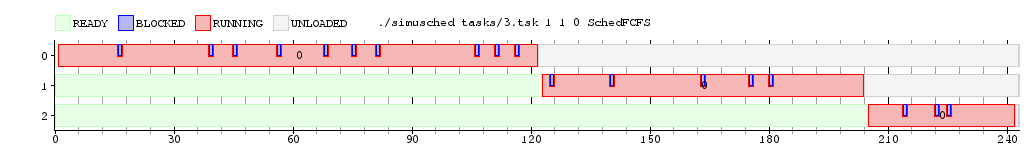
\includegraphics[width=\linewidth]{images/3.png}
    \label{fig:Task Consola}
    \caption{Task Batch}
\end{figure}

\textbf{TODO: Explicar bien el diagrama!}